\documentclass[12pt,a4paper]{article}
\usepackage[a4paper,top=1.5cm, bottom=1.5cm, left=1.5cm, right=1.5cm]{geometry}
\usepackage[T2A]{fontenc}
\usepackage[utf8]{inputenc}
\usepackage[russian]{babel}
\usepackage{amsmath}
\usepackage{amssymb}
\usepackage{graphicx}
\usepackage{floatrow}
\usepackage{booktabs}
\usepackage{wrapfig}
\usepackage{indentfirst}
\usepackage{lipsum}
\usepackage{subcaption}
\usepackage{float}
\restylefloat{table}

\newcommand{\figref}[1]{(см. рис. \ref{#1})}
\newcommand{\e}[1]{\text{$\cdot10^{#1}$}}

\title{Лабораторная работа 2.1.3\\ Определение $C_p/C_v$ по скорости звука в газе}
\author{Симанкович Александр \\ Б01-104}
\date{12.04.2022}


\begin{document}
	\maketitle
	
	\section*{Цель работы}
		
	Измерение частоты колебаний и длины волны при резонансе звуковых колебаний в газе, заполняющем трубу
	
	Определение показателя адиабаты с помощью уравнения состояния идеального газа.
	
	\section*{Оборудование и приборы} 
	Звуковой генератор ГЗ;
	электронный осциллограф ЭО;
	микрофон;
	телефон;
	раздвижная труба;
	теплоизолированная труба, обогреваемая водой из термостата;
	баллон со сжатым углекислым газом;
	газгольдер.
	
	\section*{Теоретическое введение}
	
		
	Cкорость распространения звуковой волны в газах зависит от показателя адиабаты $\gamma$.
	На измерении скорости звука основан один из наиболее  точных методов определения показателя  адиабаты.
	
	Скорость звука в газах определяется формулой:
	$$c=\sqrt{\gamma\frac{RT}{\mu}},$$
	где $R$ - газовая постоянная, $T$ - температура газа, а $\mu$ его молярная масса.
	Выразим показатель адиабаты:
	$$\gamma=\frac{\mu}{RT} c^2$$
	
	Звуковая волна, распространяющаяся вдоль трубы, испытывает многократные отражения от торцов.
	Звуковые колебания в трубе являются наложением всех отраженных волн и, вообще говоря, очень сложны.
	Картина упрощается, если длина трубы L равна целому числу полуволн, то есть когда
	$$L=n\frac{\lambda}{2},$$
	где $\lambda$ — длина волны звука в трубе, а $n$ — любое целое число.
	
	Скорость звука c связана с его частотой $f$ и длиной волны $\lambda$ соотношением:
	$$c=\lambda f.$$
	
	Подбор условий, при которых возникает резонанс, можно производить двояко:
	
	1) При неизменной частоте f звукового генератора (а следовательно, и неизменной длине звуковой волны $\lambda$) можно изменять длину трубы $L$.
	Для этого применяется раздвижная труба.
	Длина раздвижной трубы постепенно увеличивается, и наблюдается ряд последовательных резонансов.
	Для $k$-ого резонанса имеем:
	$$L_{n+k}=n\frac{\lambda}{2} + k\frac{\lambda}{2},$$
	т. е. $\lambda/2$ равно угловому коэффициенту графика, изображающего зависимость длины трубы $L$ от номера резонанса $k$.
	
	2) При постоянной длине трубы можно изменять частоту звуковых
	колебаний.
	В этом случае следует плавно изменять частоту $f$ звукового генератора, а следовательно, и длину звуковой волны $\lambda$.
	Для $k$-ого резонанса получим:
	$$L = (n+k)\frac{\lambda_{k+1}}{2}$$
	$$f_{k+1} = \frac{c}{\lambda_{k+1}}=\frac{c}{2L}(n+k)=f_1 + \frac{c}{2L}k.$$
	
	Скорость звука, деленная на $2L$, определяется, таким образом, по угловому коэффициенту графика зависимости частоты от номера резонанса.
		

	\section*{Экспериментальная установка}
	
	\begin{figure}[h]
		\caption{установка с раздвижной трубой}
		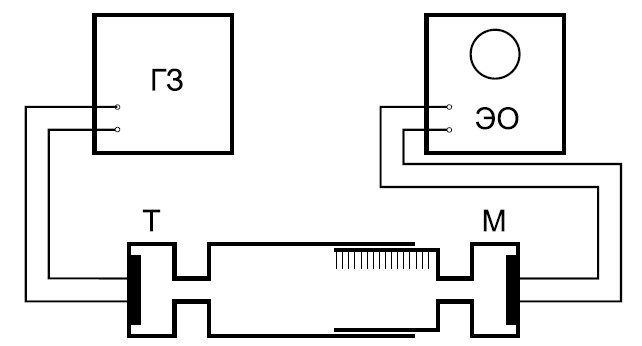
\includegraphics[scale=0.65]{scheme1.jpg}
		\label{scheme1}
	\end{figure}

	\begin{figure}[h]
		\caption{установка с термостатом}
		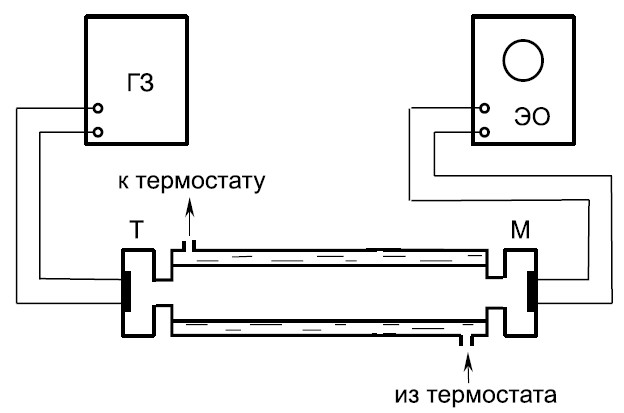
\includegraphics[scale=0.65]{scheme2.jpg}
		\label{scheme2}
	\end{figure}
	
	Соответственно двум методам измерения скорости звука в работе имеются две установки.
	В обеих установках звуковые колебания в трубе возбуждаются телефоном Т и улавливаются микрофоном М.
	Мембрана телефона приводится в движение переменным током звуковой частоты; в качестве источника переменной ЭДС используется звуковой генератор ГЗ.
	Возникающий в микрофоне сигнал наблюдается на осциллографе ЭО.
	
	Микрофон и телефон присоединены к установке через тонкие резиновые трубки.
	Такая связь достаточна для возбуждения и обнаружения звуковых колебаний в трубе и в то же время мало возмущает эти колебания: при расчетах оба торца трубы можно считать неподвижными, а влиянием соединительных отверстий пренебречь.
	
	Первая установка \figref{scheme1} содержит раздвижную трубу с миллиметровой шкалой.
	Через патрубок (на рисунке не показан) труба может наполняться воздухом или углекислым газом из газгольдера.
	На этой установке производятся измерения $\gamma$ для воздуха и для $CO_2$.
	
	Вторая установка \figref{scheme2} содержит теплоизолированную трубу постоянной длины.
	Воздух в трубе нагревается водой из термостата.
	Температура газа принимается равной температуре омывающей трубу воды.
	На этой установке измеряется зависимость скорости звука от температуры.
	
	\section*{Ход работы}
	
		\subsection*{Измерение $ C_p/C_v $ для воздуха при помощи установки с раздвижной трубой}
		
		Проведём измерение коэффициента $ C_p/C_v $ для воздуха при помощи установки с раздвижной трубой.
		Для проведения серии измерений фиксируем частоту звукового сигнала и оставляем её неизменной при до окончания снятия показаний.
		Увеличиваем и уменьшаем длину трубки, чтобы добиться резонанса, возникновение которого устанавливается при помощи осциллографа.
		При возникновении резонанса фиксируем то расстояние, на которое была выдвинута трубка прибора.
		Данные измерения проводим для нескольких значений частот.
		Полученные результаты заносим в таблицу.
		
		\begin{table}[H]
			\caption{Измерения $l(k)$ для фиксированных $f$, воздух}
			\input{L_k_air.tex}
		\end{table}
		
		Для каждого измерения удлинения трубы ошибка составляет $\sigma_l = 1.0$ мм.
		Соответственно для разности длин $\sigma_L = \sqrt{2} \sigma_l = 1.5$ мм.
		
		Построим график:
		
		\begin{figure}[H]
			\includegraphics{L_k_air.pdf}
			\caption{Зависимость $L(k)$ для воздуха}
		\end{figure}
	
		По методу наименьших квадратов рассчитаем $a$ считая зависимость линейной ($y = ax + b$).
	
		\begin{table}[h]
			\caption{Результаты вычислений для воздуха}
			\input{processed_L_k_air.tex}
		\end{table}
		
		Наклон данных графиков $a = \lambda/2$, отсюда $\lambda = 2a$.
		При этом 
			$$c = \lambda f$$
		
		Погрешность:
			$$\sigma_c = c \sqrt{\varepsilon_{\lambda}^2 + \varepsilon_{f}^2}$$
		
		Тогда, усредняя значения скорости звука при разных частотах:
			$$c = (347 \pm 5) \; \text{м/с}$$
			
		Температура, при которой проводились измерения: $T = 296$ К.
		
		Тогда
			$$\gamma = 1.42 \pm 0.04$$
		
\newpage

		\subsection*{Измерение $ C_p/C_v $ для углекислого газа при помощи установки с раздвижной трубой}
		
		Проводя аналогичные первой части измерения, получаем:
		
		\begin{table}[H]
			\caption{Измерения $l(k)$ для фиксированных $f$, углекислый газ}
			\input{L_k_carbon.tex}
		\end{table}
		
		Строим графики, обрабатываем по МНК.
		
		\begin{figure}[H]
			\includegraphics{L_k_carbon.pdf}
			\caption{Зависимость $L(k)$ для углекислого газа}
		\end{figure}
		
		\begin{table}[H]
			\caption{Результаты вычислений для углекислого газа}
			\input{processed_L_k_carbon.tex}
		\end{table}
		
		Скорость звука:
			$$c = (310 \pm 40) \; \text{м/с}$$
		
		Температура, при которой проводились измерения: $T = 296$ К.
		
		Тогда
			$$\gamma = 1.7 \pm 0.5$$
		
		\subsection*{Измерение $C_p/C_v$ для воздуха при различных температурах}
		
		Проведём измерения $C_p/C_v$ для воздуха при различных температурах.
		Для этого будем использовать трубу постоянного размера $L = $
		Для фиксированной температуры будем изменять частоту звукового сигнала, тем самым изменяя и длину волны, так, чтобы мы могли наблюдать последовательные резонансы.
		Для каждого резонанса будем фиксировать частоту, при которой он возник.
		Полученные измерения занесём в таблицу.
		
		\begin{table}[H]
			\caption{Измерения при фиксированной длине и различных температурах, воздух}
			\input{F_k.tex}
		\end{table}
		
		Строим графики, обрабатываем по МНК.
	
		\begin{table}[H]
			\caption{Результаты вычислений для воздуха}
			\input{processed_F_k.tex}
		\end{table}
		
		\begin{figure}[H]
			\includegraphics{F_k.pdf}
			\caption{Зависимость $F(k)$ для воздуха}
		\end{figure}
		
		Используя $a = \frac{c}{2L}$ получим значения $c$.
		Рассчитаем $\gamma$ для каждой серии измерений.
		
		Усредняя по всем сериям получим:
			$$\gamma = (1.362 \pm 0.015)$$
		
		Построим также график $c(\sqrt{T})$:
		
		\begin{figure}[H]
			\includegraphics{c_sqrt_T.pdf}
			\caption{Зависимость $c(\sqrt{T})$ для воздуха}
		\end{figure}
		
		
	\section*{Вывод}
	
		Результаты измерений в части с воздухом и раздвижной трубой хорошо описываются теорией и сходятся с табличными:
		
		$$\gamma = 1.42 \pm 0.04 \qquad \gamma_{\text{табл}} = 1.398$$
		
		Измерения, полученные в части с углекислым газом нерепрезентативны, поскольку измерения проводились при отсутствии подачи углекислого газа, использовался газ, оставшийся в трубе (запас газа в газгольдере был израсходован).
	
		Зависимость $F(k)$ в эксперименте с изменяющейся температурой хорошо описывается теорией, значения скоростей и $\gamma$ близки к табличным. 
		
		$$\gamma = 1.362 \pm 0.015 \qquad \gamma_{\text{табл}} = 1.398$$
		
		Предполагаемая линейность зависимости $c(\sqrt{T})$ также выполняется.
		
\end{document}